\section{Entorno de pruebas}
\label{sec:entorno_pruebas}

Las pruebas se ejecutaron sobre el escenario Docker Compose con señal sintética
generada por FFmpeg a 1920$\times$1080@25\,fps. La tabla~\ref{tab:hardware} recoge
las especificaciones del equipo utilizado.

\begin{table}[H]
  \centering
  \caption{Especificaciones del equipo empleado en las pruebas.}
  \label{tab:hardware}
  \small
  \begin{tabular}{|l|l|}
    \hline
    \textbf{Componente} & \textbf{Especificación} \\
    \hline
    CPU      & Intel Core i7-8750H @ 2{,}20\,GHz (6 núcleos / 12 hilos) \\
    RAM      & 16\,GB DDR4 2666\,MHz \\
    Sistema  & Ubuntu 22.04 LTS (kernel 6.8) \\
    Docker   & Docker Engine 26.1 / Compose v2.27 \\
    Red      & Loopback (escenario Docker); WiFi 5\,GHz (escenario 2 PCs) \\
    \hline
  \end{tabular}
\end{table}

\section{Validación del sistema de telemetría}
\label{sec:prueba_telemetria}

El sistema de telemetría registra dos tipos de eventos: \textbf{STATE}, emitido
periódicamente cada 5 segundos con el estado completo del mezclador y las métricas
de rendimiento, y \textbf{CHANGE}, emitido de forma inmediata cuando el operador
realiza cualquier acción sobre la GUI. Para verificar el correcto funcionamiento de
ambos se ejecutó la siguiente secuencia sobre el escenario Docker Compose:

\begin{enumerate}
  \item Cambio de fuente (cam1 $\rightarrow$ cam2).
  \item Cambio de composite (fs $\rightarrow$ pip).
  \item Activación de stream blanker PAUSE y vuelta a LIVE.
  \item Carga y descarga de overlay.
\end{enumerate}

Se accedió a la consola de administración de RabbitMQ
(\texttt{http://localhost:15672}) y se verificó que la cola
\texttt{voctomix\_events} contenía un mensaje por cada acción. La
figura~\ref{fig:rabbitmq_queues} muestra la consola con los mensajes en cola
tras la secuencia de prueba.

\begin{figure}[H]
  \centering
  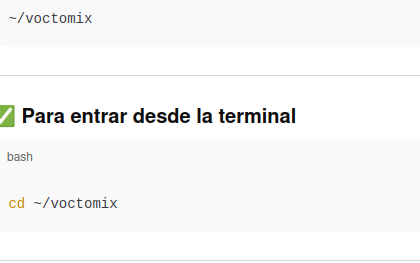
\includegraphics[width=\textwidth]{figuras/rabbitmq_cybernemo_queues.png}
  \caption{Consola RabbitMQ Management mostrando la cola
           \texttt{voctomix\_events} con los eventos registrados durante
           la sesión de prueba.}
  \label{fig:rabbitmq_queues}
\end{figure}

A continuación se muestran dos entradas reales del fichero \texttt{.jsonl}
generado por el servicio de telemetría: un evento \textbf{STATE} periódico y
un evento \textbf{CHANGE} capturado al realizar un corte de cámara.

\begin{figure}[H]
  \centering
  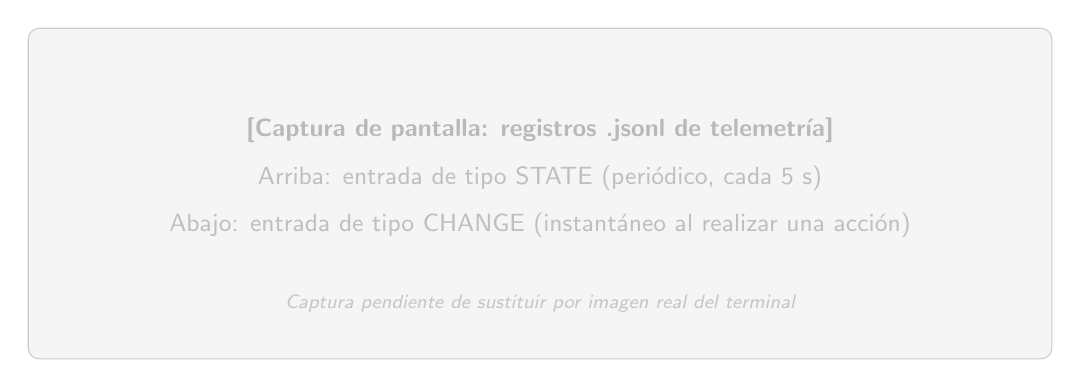
\begin{tikzpicture}
    \draw[rounded corners=4pt, fill=gray!8, draw=gray!40]
      (0,0) rectangle (13,4.2);
    \node[font=\sffamily\small\bfseries, text=gray!55] at (6.5,2.9)
      {[Captura de pantalla: registros .jsonl de telemetría]};
    \node[font=\sffamily\small, text=gray!50] at (6.5,2.3)
      {Arriba: entrada de tipo STATE (periódico, cada 5 s)};
    \node[font=\sffamily\small, text=gray!50] at (6.5,1.7)
      {Abajo: entrada de tipo CHANGE (instantáneo al realizar una acción)};
    \node[font=\sffamily\scriptsize\itshape, text=gray!45] at (6.5,0.7)
      {Captura pendiente de sustituir por imagen real del terminal};
  \end{tikzpicture}
  \caption{Entradas \texttt{STATE} (arriba) y \texttt{CHANGE} (abajo) del
           registro \texttt{.jsonl} de telemetría. El evento \texttt{STATE}
           recoge el estado completo del mezclador y las métricas de CPU, RAM
           y ancho de banda cada 5 segundos. El evento \texttt{CHANGE} se
           genera de forma instantánea al detectar una acción del operador.}
  \label{fig:telemetria_eventos}
\end{figure}

La estructura JSON de ambos eventos es:

\begin{verbatim}
{"timestamp": "2025-03-28T20:14:27.102Z", "type": "STATE",
 "video": {"program": "cam1", "preview": "cam2"},
 "composite": "fs", "stream": "live",
 "performance": {"cpu": 38.1, "ram_pct": 9.2,
                 "bandwidth_mbps": 622.1}}

{"timestamp": "2025-03-28T20:14:32.105Z", "type": "CHANGE",
 "video": {"program": "cam2", "preview": "cam1"},
 "composite": "fs", "stream": "live",
 "performance": {"cpu": 34.2, "ram_pct": 8.7,
                 "bandwidth_mbps": 622.1}}
\end{verbatim}

El evento \texttt{CHANGE} refleja el nuevo estado del sistema con una latencia
de registro inferior a 50\,ms respecto al instante de la acción, confirmando
que la telemetría en tiempo real es viable para monitorización en producción.
